\usepackage{graphicx}

\section{Miscellanea}

\subsection{Heterogeneous Aspect}

In addition to the Built-In Aspect, we are architecting a novel variant, termed as the Heterogeneous Aspect, to facilitate heterogeneous computing on the blockchain. Heterogeneous computing implies native applications cultivated based on operating systems, thus exploiting operating system resources, network requests, and an array of software utilities to construct sophisticated application logic. Presently, heterogeneous computing is primarily achieved via off-chain computations, including off-chain oracles.

This design addresses the inherent limitations of the Built-in Aspect. Operating within a virtual machine, the Built-in Aspect necessitates deterministic execution, resulting in confined resource access. On the other hand, the Heterogeneous Aspect is granted network access, enabling it to undertake demanding computational tasks. For example, running AI models, which are resource-intensive and yield non-deterministic execution results, might not be viable on virtual machines. However, these tasks are feasible within the Heterogeneous Aspect's framework.

The Heterogeneous Aspect, inherently a native application, is encapsulated within containers. This approach affords an expansion in the technological repertoire of the decentralized sphere by integrating advancements such as artificial intelligence, privacy computation, real-time computation, and decentralized storage. Heterogeneous Aspect's deployment and execution are handled within a heterogeneously architected computing network, a network that shares security in mutual accordance with the main network.

The differences between Built-in Aspects and Heterogeneous Aspects are shown in the table:

\begin{table}[htbp]
    \centering
    \begin{tabular}{|l|p{6cm}|p{6cm}|}
      \hline
      & Built-in Aspect & Heterogeneous Aspect \\
      \hline
      Consensus mechanism & Loaded and executed by main net validator nodes & Can be executed by heterogeneous computing nodes, and shares security with main net validation nodes \\
      \hline
      Execution environment & Executed in a deterministic sandbox environment & Supports interaction with external heterogeneous computing platforms and external networks \\
      \hline
      Runtime restrictions & Provides limited Runtime APIs, no IO/thread/async operation/network and other high-uncertainty operation capabilities & Native program, not limited by its execution capabilities \\
      \hline
    \end{tabular}
  \end{table}
  


\subsection{Difference Between Aspect and Off-chain Computation}

Off-chain computation refers to a model similar to Oracle, where computations occur on an off-chain consensus network. The consensus is reached off-chain on the calculated results before these are input into smart contracts for utilization.
The distinctions between Aspect and off-chain computation encompass:

\begin{itemize}
  \item \textbf{Security:} Relative to L1, the contrast between Aspect and off-chain computation parallels the differences between rollup and side-chain. While one shares security with the main network, the other assumes responsibility for its security.
  \item \textbf{Interoperability:} Both Aspect and off-chain computation exhibit interoperability with contracts on L1, similar to the interoperability seen within intra-chain contract interactions and across different chains. Aspect and contract execution occur synchronously within the same transaction, whereas off-chain computation and contracts establish a distributed transaction and are typically asynchronous.
  \item \textbf{Characteristics:} As an on-chain native program, Aspect forms part of the consensus process. It can operate within the context of the consensus execution process, such as customizing transaction data structures, validating methods, and appending additional transactions.
\end{itemize}

In conclusion, Aspect and off-chain computation can act as synergistic complements to each other, empowering both smart contracts and applications. However, due to its native extension features, Aspect possesses unique functionalities that off-chain computation cannot replicate.

\subsection{About Latency Problem}

Transactions executing both a smart contract and an Aspect may exhibit elevated latency in comparison to those executing a smart contract alone. It is critical to distinguish between the following two scenarios:

\begin{enumerate}
  \item \textbf{Embedding a specific logic in an Aspect for an existing smart contract.} In the absence of an Aspect, this particular logic could be executed within off-chain components, thus not contributing to increased on-chain latency. However, if we shift this logic from off-chain components to on-chain Aspects, the transaction latency would escalate.
  \item \textbf{Implementing specific functionality via an EVM-based smart contract augmented by a WASM-based Aspect.} Were this specific functionality to be implemented exclusively by the EVM-based smart contract, transaction calls to this functionality would exhibit increased latency, as the WASM-based Aspect executes at a faster rate than the smart contract. In this scenario, the Aspect mitigates the latency.
\end{enumerate}

Despite these two scenarios seemingly contradicting each other, it is a fallacy to assume that Aspects inherently increase latency. The latency is predominantly determined by the transaction's gas limit. Given the same latency, transactions executed through an Aspect can utilize more gas.

To rigorously appraise the execution overhead associated with Aspect, and to fine-tune the balance between the computational potentials of EVM and ArtWASM, a meticulous sequence of tests were anchored around the Fibonacci algorithm.

The experimental context was articulated as follows:

\begin{enumerate}
  \item ArtWASM's runtime, crafted in Go 1.21, employs WASMTime v11.0.0 as its pivotal execution engine.
  \item The testing was facilitated on a machine powered by a 2.2 GHz Haswell CPU.
  \item The referential smart contract was sculpted using Solidity version 0.8.20, setting it in contrast with the Aspect test code, designed in Assembly Script 0.27.5.
  \item To preserve the experiment's integrity, both Solidity and Assembly Script were devoid of optimizations, with Aspect's code strictly compiled under the -O0 flag. A thorough validation of the ensuing .wat file ensured an absence of compiler-infused enhancements.
\end{enumerate}

Three discerning tests were architected to identify the interplay between join-points and performance dynamics:

\begin{enumerate}
  \item The initial test, embodied in the leftmost figure, constrained join-points to 10, while sequentially amplifying Fibonacci iterations. This aimed at highlighting the juncture where Aspect's efficiency eclipses that of traditional smart contracts.
  \item The next test, showcased in the central figure, spun 1600 Fibonacci iterations across both EVM and ArtWASM platforms, reiterated 100,000 times. This setup progressively augmented the count of join-points, enabling a nuanced correlation study between ArtWASM and EVM execution trajectories.
  \item The final test, encapsulated in the rightmost figure, established an execution time ceiling (1 milli-second), and concurrently augmented join-points. This test endeavored to reveal the computational headroom ArtWASM holds over EVM.
\end{enumerate}

\begin{figure}[htp]
  \centering
  \begin{minipage}{0.3\textwidth}
    \centering
    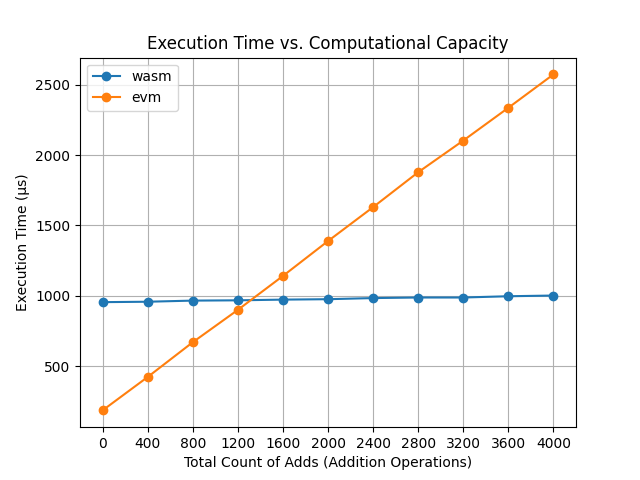
\includegraphics[width=1\linewidth]{sections/tx-latency-et-vs-cc.png}
    \caption{Equilibrium Analysis between Aspect and Smart Contract Computation}
    \label{fig:image1}
  \end{minipage}\hfill
  \begin{minipage}{0.3\textwidth}
    \centering
    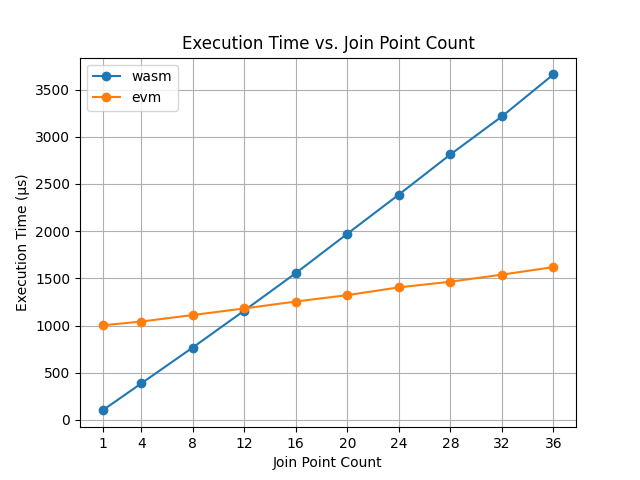
\includegraphics[width=1\linewidth]{sections/tx-latency-et-vs-jpc.png}
    \caption{Performance Interrelation between ArtWASM and EVM}
    \label{fig:image2}
  \end{minipage}\hfill
  \begin{minipage}{0.3\textwidth}
    \centering
    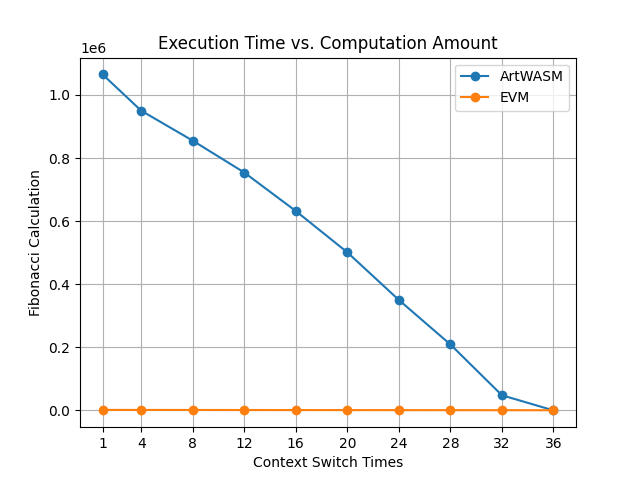
\includegraphics[width=1\linewidth]{sections/tx-latency-na-vs-jpc.png}
    \caption{Performance Delineation of ArtWASM and EVM}
    \label{fig:image3}
  \end{minipage}
\end{figure}

Drawing insights from the data, we can sculpt equations detailing the execution costs for both ArtWASM and EVM:

\[
\text{ArtWASM Execution Total Time} \equiv 29.5 \times \text{Number of Join Points} + \text{Execution Time}
\]
\[
\text{EVM Execution Total Time} \equiv 18.8 \times \text{Number of Calls} + \text{Execution Time}
\]

With an exhaustive examination of 6,000 contemporary Ethereum blocks, the average transactional gas consumption is around 280,079.07. Fascinatingly, this aligns with the gas demands of Fibonacci(1600), estimated at 280,255. Marrying this computational weight of Fibonacci(1600) with test data revealed a stark performance disparity between EVM and ArtWASM:

\[
  \frac{\text{EVM Performance}}{\text{ArtWASM Performance}} \approx \frac{1}{2026}
\]

From the Figure 5 (the second test), we can observe that when context switch time is 32, the execution time is about the same as a single EVM call. Which means if we modularize the dApp and migrate the logics from smart contract to Aspect, it is recommanded that the number of join-points used to be less than 32.

The last test emphasizes that, given the pronounced performance chasm between EVM and ArtWASM, the convergence point of the trajectories is at 33 join-points. This implies that for a transaction execution window of 1ms, the upper bound for join-points stands at 33.

The gleaned insights coalesce into several pivotal conclusions:

\begin{enumerate}
  \item Contextual switches between join-points induce a bit more overhead than an EVM call.
  \item ArtWASM's computational prowess markedly overshadows that of the EVM.
  \item It's economically prudent to nestle intricate logic within Aspect, relegating simpler logic to the smart contract.
  \item Pruning the number of join-points harnessed yields cost efficiencies.
\end{enumerate}

Distilling the insights, we can encapsulate the dynamics in the equation:

\[
  \text{ExtraComputationCapacity} \equiv \frac{\text{AspectExecTime} - \text{ContextSwitchLatency} \times \text{JoinPointNumber}}{\text{EVMExecutionLatency} \times \frac{1}{2026}}
\]

It is recommanded to adjust the Aspect execution latency dynamically for the given blockchain platform. For example, in harmony with prevailing usage patterns, we postulate:

\begin{enumerate}
  \item Aspect aims to accommodate transaction execution latencies with a moderate 65\% uptick.
  \item Of this latency, 45\% is earmarked for context switching.
  \item The residual 20\% is allocated for execution.
\end{enumerate}

Leveraging the aforementioned postulates and empirical findings, and with Ethereum's average transaction latency as our baseline, our assumptions suggest that up to 15 join-points can be executed per transaction, heralding a monumental 40000\% surge in execution performance for the system. This is just a theoretical assumption specifically for Artela, and the actual number of join-points should be adjusted according to the actual blockchain platform.
